\renewcommand{\lastmod}{8. Oktober 2024}
\renewcommand{\chapterauthors}{Markus Lippitz}

\chapter{Die Grenzen der klassischen Physik}


\section{Überblick}

In diesem Kapitel geht es um den Aufbau und die Eigenschaften von Atomen. Atome entziehen sich unserer Anschauung. Wir können sie nicht direkt erfahren. Wir können nur die Ergebnisse von Experimenten beobachten und versuchen, daraus Schlüsse zu ziehen. Daraus entwickeln wir ein physikalisches Modell, das aber eigentlich nur in unserer Vorstellung existiert. In diesem Kapitel geht es daher viel darum, welche experimentellen Beobachtungen mit welcher Vorstellung noch vereinbar sind oder wie man das Modell anpassen muss, um das Experiment beschreiben zu können. Wir folgen hier der erkenntnisgeschichtlichen Entwicklung gegen Ende des 19.

\vspace*{\parskip}

Wir diskutieren vier Bereiche
\begin{itemize} \setlength{\itemsep}{0pt}
    \item Wie kann man mit Licht etwas über einen Objekt erfahren? Heiße Körper emittieren ein kontinuierliches Spektrum, atomare Gase dagegen diskrete Linien.
    \item Woher wissen wir, dass Atome aus noch kleineren Teilchen aufgebaut sind? Die Elektronenstrahlröhre ermöglichte wichtige Experimente.
    \item Wie konnte das Rutherfordsche Streuexperiment zeigen, dass sich die gesamte Masse eines Atoms im Kern befindet?
    \item Woraus besteht dieser Kern?
\end{itemize}


Dieses Kapitel entspricht in seinem Aufbau dem Kapitel 37 von \cite{Knight_physics}. Gute andere Darstellungen finden sich in \cite{Haliday_Resnick}, \cite{Demtröder_ep3} und \cite{Haken_wolf_I}.





\section{Was bislang geschah}

Die Vorstellung, dass Materie aus nicht weiter teilbaren Teilchen, den Atomen, besteht, geht auf die griechischen Philosophen Leukipp und Demokrit im 5. Jahrhundert vor Christus. 'Atomos' ist griechisch und bedeutet 'unteilbar'. Das war aber nur eine Vorstellung, die durch keine Beobachtung gestützt wurde.

In der Chemie konnte John Dalton um 1808 zeigen, dass chemische Reaktionen gut verstanden werden können, wenn man von ganzzahligen Verhältnissen der beteiligten Elemente ausgeht ('Gesetz der multiplem Proportionen'). Abweichungen vom idealen Gasgesetz lassen Rückschlüsse auf die Größe der Atome zu.

Licht wurde seit dem Doppelspaltexperiment von Thomas Young (1801) als Welle verstanden und schließlich von  James Clerk Maxwell 1862 als elektromagnetische Welle beschrieben.

Als Max Planck sich um 1874 für ein Physikstudium interessierte, sagte ihm der Münchner Physikprofessor Philipp von Jolly, dass eigentlich schon alles erforscht sei und es keine wesentlichen Fragen mehr gäbe.

Eine Reihe von Experimenten zeigte Ende des 19. Jahrhunderts Widersprüche zu den bis dahin gültigen Modellen auf. Diese Experimente zum Aufbau der Atome und zur Natur des Lichts begründeten die 'Moderne Physik'. Auch wenn wir Atome nicht direkt sehen können, so können wir doch aus verschiedenen Experimenten Rückschlüsse auf ihren Aufbau ziehen.

\section{Schwarzkörperstrahlung}

\begin{marginfigure}
    \inputtikz{\currfiledir planck_linlog}
    \caption{Schwarzkörperspektren. Oben: lineare Darstellung für $T=$ 3000 K, 4000 K und 5000 K. Unten: Doppelt-logarithmische Darstellung (3000 K) mit Modellen von Wien und Rayleigh-Jeans.}
    \label{fig:1_planck_linlog}
\end{marginfigure}


Wichtige Erkenntnisse über die Natur des Lichts stammen aus einer einfachen Beobachtung: Viele leuchtende Objekte ändern ihre Farbe in Abhängigkeit von der Temperatur. Der Glühfaden einer Glühbirne ändert seine Farbe von grau zu gelb, wenn er durch den fließenden Strom nur heiß genug wird. Stahl ändert seine Farbe im Kohlefeuer der Schmiede. Lava ist im kalten Zustand schwarz, am Vulkan aber rot bis gelb.

In der Wärmelehre haben Sie gesehen, dass die Wärmestrahlung eines Körpers mit der vierten Potenz seiner Temperatur $T$ zunimmt
\begin{equation}
    \dot{Q} = e \, \sigma \, A \, T^4
\end{equation}
mit der Emissivität $e$, der Stefan-Boltzmann-Konstanten $\sigma$ und der Objektoberfläche $A$. Die Emissivität $e$, auch Emissionsgrad genannt, ist eins für einen idealen Wärmestrahler. Dieser wird als Schwarzkörper und das von ihm abgestrahlte Licht als Schwarzkörperstrahlung bezeichnet.

Ende des 19. Jahrhunderts versuchte man, möglichst ideale Schwarzkörper zu konstruieren und deren Emissionsspektren möglichst genau zu messen. Abbildung  \ref{fig:1_planck_linlog} zeigt Schwarzkörperspektren für verschiedene Temperaturen. Mit steigender Temperatur nimmt die spektrale Intensität bei jeder Wellenlänge zu. Gleichzeitig verschiebt sich das Maximum zu kurzen Wellenlängen, entsprechend dem \emph{Wien'schen Verschiebungsgesetz}
\begin{equation}
    \lambda_{peak} = \frac{b}{T}
\end{equation}
mit der Wien'schen Verschiebungskonstanten $b \approx $ 2898 \textmu m K .

Damals erwartete man, dass die Form des Schwarzkörperspektrums aus einer gut verstandenen Thermodynamik und der Maxwellschen Theorie der elektromagnetischen Strahlung abgeleitet werden könnte. Man fand zwei Modelle\sidenote{Wir diskutieren im nächsten Kapitel die heute akzeptierte Form und finden dann diese beiden alten Modelle als Genzfälle}, die aber jeweils nur einen Teil des Spektrums richtig beschrieben: Das Wiensche Gesetz den langwelligen Teil, das von Rayleigh und Jeans den kurzwelligen. Schlimmer noch: Das Rayleigh-Jeans-Gesetz liefert ein divergierendes Spektrum, so dass auch die abgestrahlte Leistung divergiert. Das ist die \emph{UV-Katastrophe}.

Trotz des einfachen Experiments 'Spektrum eines schwarzen Körpers' und eigentlich gut verstandener Theorien zur Elektrodynamik und Thermodynamik funktioniert hier also etwas nicht.


\paragraph*{Spektren über der Wellenlänge und über der Frequenz} Ich zeige hier nur Spektren über der Wellenlänge $\lambda$. Mit $\nu = c / \lambda$ kann man auch zur Frequenz $\nu$ übergehen. Dabei ändert sich aber nicht nur die x-Achse, sondern auch der y-Wert des Spektrums, da eigentlich $I(\lambda) d\lambda$ bzw. $I(\nu) d\nu$ aufgetragen wird und somit auch $d\lambda$ in $d\nu$ umgerechnet werden muss. Dies wird besonders deutlich, wenn man bedenkt, dass das Integral über das Spektrum unabhängig von der Skalierung der x-Achse immer die gleiche Leistung ergeben muss. Bei dieser Umrechnung ändert sich die Form des Spektrums und damit die Lage des Maximums, also 
\begin{equation}
    \nu_{peak} \neq \frac{c}{\lambda_{peak}} \quad .
\end{equation}


\begin{questions}  
\item Sonnenlicht lässt sich gut durch ein Schwarzkörperspektren von etwa 5000~K beschrieben. Die Erde hingegen strahlt wie ein Körper von 300~K in den Weltraum ab. Skizzieren Sie diese beiden Spektren und leiten Sie daraus das Transmissionsspektrum der Atmosphäre ab, das zum natürlichen Treibhauseffekt führt.
\end{questions}


\section{Spektren von atomaren Gasen}

In einer Gasentladungsröhre fließt ein elektrischer Strom durch ein Gas, das in einer Glasröhre eingeschlossen ist. Die bunten Lichter der Leuchtreklame oder 'Neonröhren' basieren auf diesem Prinzip, haben aber manchmal noch einen leuchtenden Phosphor als Beschichtung auf der Röhre selbst. Das Emissionsspektrum unterscheidet sich deutlich von dem eines schwarzen Strahlers. Es besteht aus diskreten, sehr scharfen Linien, die sich für jedes Element wie ein Fingerabdruck unterscheiden. Neon zum Beispiel hat viele Linien im roten Spektralbereich (Abb.~\ref{fig:1:Ne_linien} oben). Sie erzeugen das rote Licht der Leuchtreklame.

\begin{marginfigure}
    \ Emission

    \pgfspectra[width=\textwidth ,element=Ne , Imin=0.2]
% 540.1 585.2 640.2 692.9 702.4 703.2 717.4 724.5 748.9 753.6
% \pgfspectradata{element=Ne, Imin=0.2}  \pgfspectratable

    \ \\

   \  Absorption

   % from DOI: 10.21883/EOS.2022.14.53991.2177-21
   \pgfspectra[width=\textwidth ,absorption, lines={585.2  , 692.9}]

\caption{Spektrallinien von \ch{Ne} in Emission und Absorption.}
\label{fig:1:Ne_linien}
\end{marginfigure}

Man kann auch das Absorptionsspektrum der Atome eines Gases messen, indem man beispielsweise ein kontinuierliches Schwarzkörperspektrum durch ein Gas schickt und dann spektroskopiert. Man findet diskrete, schmale, dunkle Linien, die das Gas aus dem breiten Spektrum des Schwarzkörpers herausschneidet  (Abb.~\ref{fig:1:Ne_linien} unterschiedlichen). Diese Absorptionslinien sind jedoch nur eine Teilmenge der Emissionslinien. Für jede Absorptionslinie gibt es eine Emissionslinie bei der gleichen Wellenlänge, aber nicht umgekehrt.

Mit der klassischen Physik war das alles nicht zu erklären. Warum diskrete Linien, warum für jedes Element anders, warum mehr in der Emission als in der Absorption?


\begin{figure}
    \pgfspectra[width=\textwidth, element=H,back=visible40, gamma=.6,axis, axis step=50,axis ticks=4,begin=300,end=750,
    axis label text={Wellenlänge $\lambda$ (nm)},axis label position=right, UVcolor=white, IRcolor=white]
    
    \caption{Die Balmer-Serie von Wasserstoff.}
    \label{fig:1_balmer}
    \end{figure}

Der einzige Lichtblick war die Entdeckung des Schweizer Lehrers Johann Balmer, dass die Wellenlänge der Emissionslinien des einfachsten Atoms, des Wasserstoffs, durch eine einfache Formel beschrieben werden kann:
\begin{equation}
    \lambda = \frac{\SI{91.18}{nm}}{ 
       \frac{1}{m^2} - \frac{1}{n^2} 
    }
    \quad \text{mit} \quad m = 1,2, 3, \dots \quad \text{und} \quad n = m+1, m+2, \dots
\end{equation}
Diese \emph{Balmer-Formel} beschreibt für $m=2$ die zuerst beobachtete \emph{Balmer-Serie}, eine Abfolge von Linien im sichtbaren Spektralbereich, die immer enger zusammenrücken und gegen 365~nm konvergieren (Abb. \ref{fig:1_balmer}).

Die Balmerformel ist rein empirisch. Die zufällig gefundene Kombination ganzer Zahlen liefert die Position der Linien. Worauf sie beruht, ist zu diesem Zeitpunkt noch völlig unklar. Eine so einfache Beziehung sollte eigentlich eine einfache Begründung haben.


\section{Kathodenstrahlen}

Mit zunehmender Verbesserung der Vakuumtechnik ist aufgefallen, dass in Gasentladungsröhren nicht nur das Gas in einer für das Gas charakteristischen Farbe leuchtet, sondern auch Teile der Glasröhre grünlich leuchten.  Von der Kathode scheinen Strahlen auszugehen, die sich geradlinig ausbreiten. Gegenstände im Strahlengang werfen einen Schatten. Diese Strahlen nannte man Kathodenstrahlen.

\begin{marginfigure}
    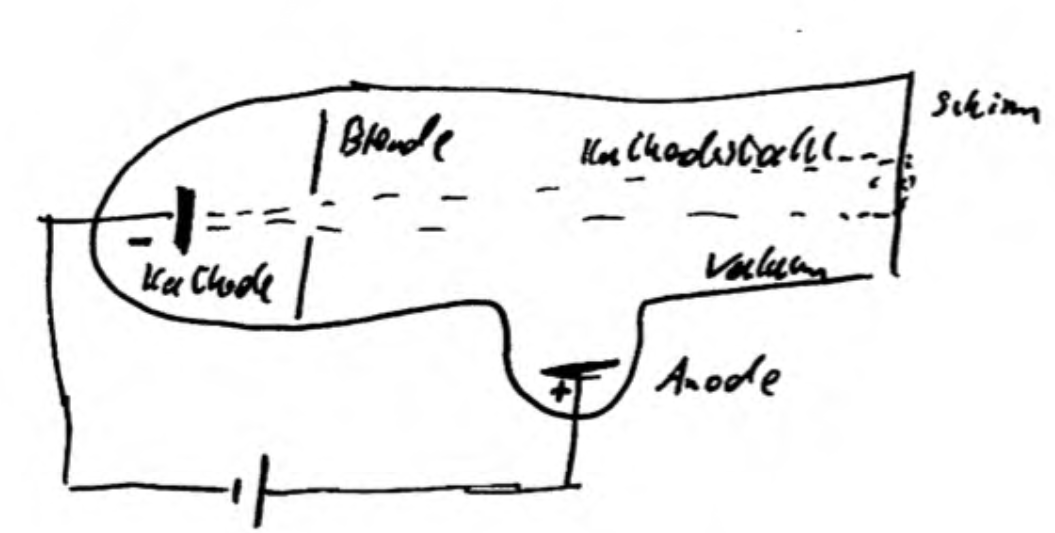
\includegraphics[width=\textwidth]{\currfiledir sketch/kathodenstrahlen.png}
    \caption{Aufbau einer Kathodenstrahl-Röhre}
\end{marginfigure}

William Crookes und andere entdeckten Ende des 19. Jahrhunderts, dass Kathodenstrahlen mit einem elektrischen Strom in der Gasentladungsröhre zusammenhängen. Die Strahlen werden durch ein Magnetfeld abgelenkt, als wären sie negativ geladen. Und die Strahlen sind unabhängig vom Material der Kathode.

Geladene Gasteilchen könnten eine Erklärung sein. Ihre mittlere freie Weglänge ist aber viel kleiner als die Länge der Röhre. Sie müssten sehr oft zusammenstoßen und könnten sich nicht geradlinig ausbreiten.

Maxwells Theorie der elektromagnetischen Strahlung war damals noch sehr jung. Man wusste, dass sich Licht nicht von Magnetfeldern ablenken lässt. Man konnte aber nicht ganz ausschließen, dass Strahlung mit einer ganz anderen Wellenlänge abgelenkt werden könnte.


\begin{marginfigure}
    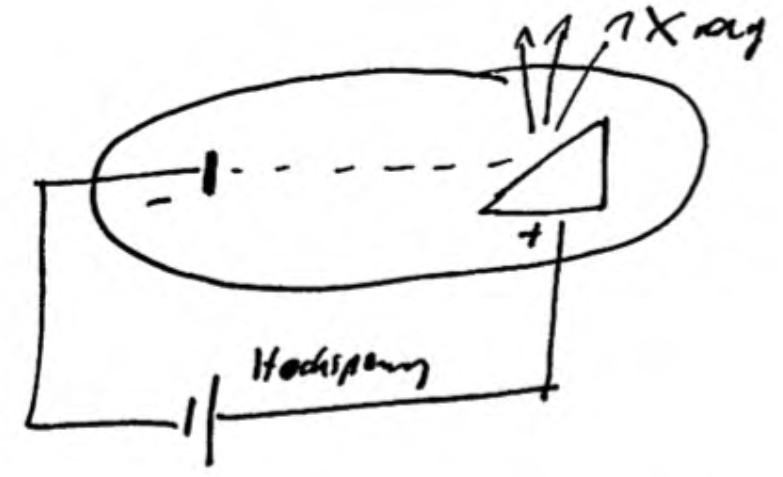
\includegraphics[width=\textwidth]{\currfiledir sketch/xray.png}
    \caption{Aufbau einer Röntgen-Röhre}
\end{marginfigure}

Wilhelm Röntgen untersuchte diese Kathodenstrahlen. Er entdeckte 1895, dass eine andere Art von Strahlung entsteht, wenn die Kathodenstrahlen auf eine Metallanode treffen. Diese später als Röntgenstrahlung bezeichnete Strahlung verlässt die Entladungsröhre, durchdringt praktisch alle Materialien und belichtet Filme. Erst später wurden Röntgenstrahlen als sehr kurzwellige elektromagnetische Wellen erkannt, die ebenfalls den Maxwell-Gleichungen unterliegen.

Joseph John Thomson schließlich hatte die Idee, die Kathodenstrahlen in einem Magnetfeld so abzulenken, dass sie auf eine Anode treffen. Nur in diesem Fall fließt ein Strom durch die Anode, nicht aber, wenn der Kathodenstrahl auf die daneben liegende Glaswand trifft. Damit war bewiesen, dass der Strahl aus negativ geladenen Teilchen besteht.

\begin{marginfigure}
    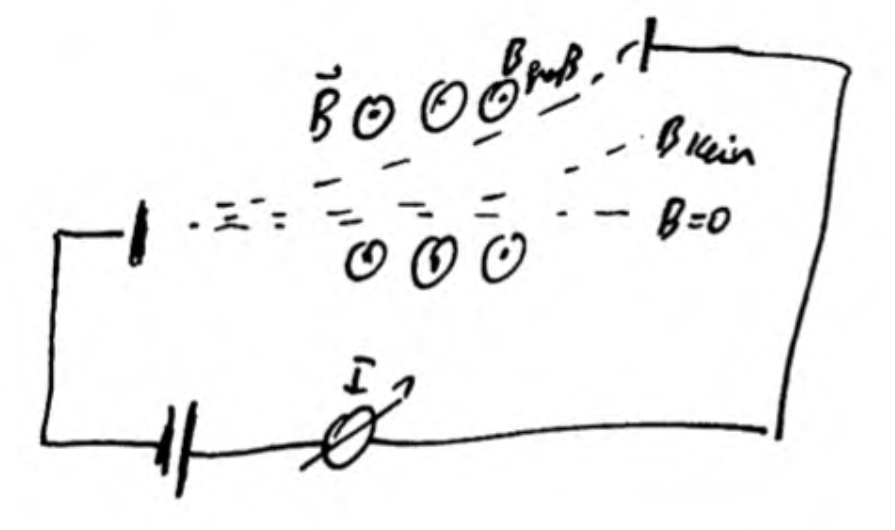
\includegraphics[width=\textwidth]{\currfiledir sketch/kathodenstrahl_bfeld.png}
    \caption{Ablenkung von  Kathodenstrahlen im Magnetfeld}
\end{marginfigure}


\section{Gekreuzte E- und B-Felder}

Die Ablenkung einer Ladung $q$ mit der Geschwindigkeit $v$ in einem Magnetfeld $B$ aufgrund der Lorentzkraft
\begin{equation}
    F_B = q \, v \, B
\end{equation}
führt zu einer Kreisbahn mit dem Radius $r$
\begin{equation}
    r = \frac{m v}{q B}
\end{equation}
mit der Masse $m$ des Teilchens. Die Ablenkung im Magnetfeld hängt also von zu vielen Unbekannten ab, um eine Aussage über das Teilchen machen zu können.


\begin{marginfigure}
    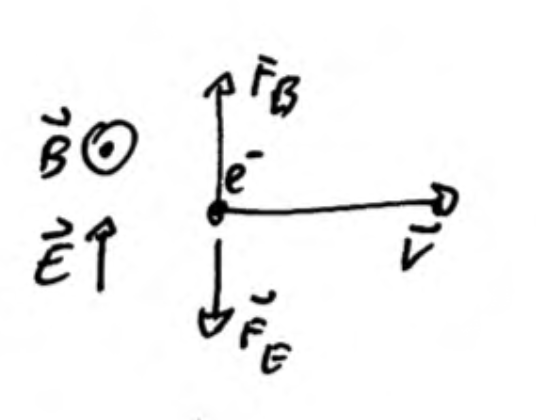
\includegraphics[width=\textwidth]{\currfiledir  sketch/kraefte_bfeld.png}
    \caption{Kräfte auf eine bewegte Ladung}
\end{marginfigure}


J.J. Thomsons Idee war, gleichzeitig ein elektrisches Feld $E$ senkrecht zum B-Feld anzulegen. Die Coulombkraft wirkt dann der Lorentzkraft entgegen und kann die Ablenkung kompensieren. Für den Fall der geradlinigen Ausbreitung gilt daher
\begin{equation}
    F_B = q v B = q E = F_E  \quad \text{bzw.} \quad v = \frac{E}{B}  \quad .
\end{equation}
Damit kann die Geschwindigkeit $v$ bestimmt werden. Bleibt dann alles unverändert, wird nur das E-Feld abgeschaltet, so kann mit der nun bekannten Geschwindigkeit $v$ aus der Kreisbahn das Ladungs-Masse-Verhältnis bestimmt werden
\begin{equation}
    \frac{q}{m} = \frac{v}{r B}  \quad .
\end{equation}



\section{Das Elektron}

J.J. Thomson fand\sidenote{heutiger Wert des Elektrons $q/m \approx 1.76 \cdot 10^{11}$C/kg} für die Teilchen im Kathodenstrahl $q/m \approx 1 \cdot 10^{11}$C/kg, etwa 1000 mal größer als der aus der Elektrolyse bekannte Wert des Wasserstoffions. Aber ob die Masse kleiner oder die Ladung größer war als beim Wasserstoffion oder beides, konnte nicht gesagt werden. Man vermutete aus der Elektrolyse, dass die Ladung quantisiert ist, aber der Zusammenhang zwischen Kathodenstrahl und Elektrolyse war nicht offensichtlich. Thomson argumentierte, dass Kathodenstrahlen dünne Metallfilme durchdringen können, Atome jedoch nicht. Daher müssten die Kathodenstrahlen aus viel kleineren Teilchen bestehen, die wiederum Bestandteil des Atoms sind. Diese Teilchen wurden später als Elektronen bezeichnet.

\section{Millikans Öltröpfchen-Experiment: die Elementarladung}

\begin{marginfigure}
    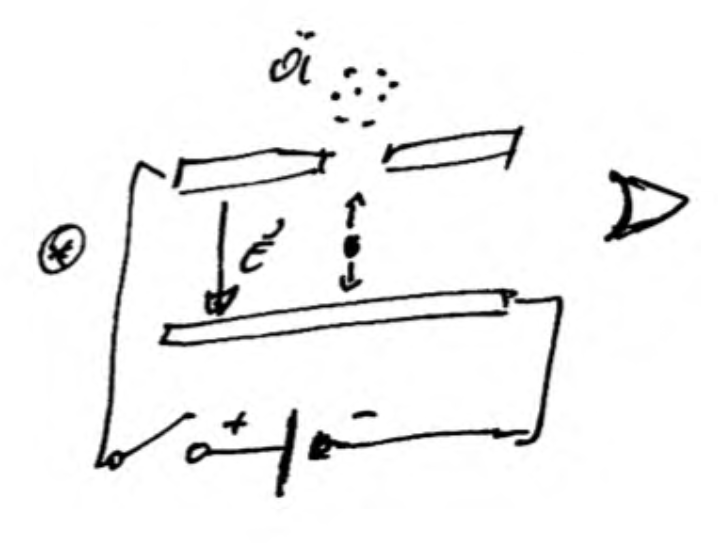
\includegraphics[width=\textwidth]{\currfiledir  sketch/millikan.png}
    \caption{Skizze des Aufbaus von Millikan}
\end{marginfigure}



Thomson hatte das Verhältnis $q/m$ bestimmt, aber nicht die Bestandteile aufgelöst. Dies gelang 1906 Robert Millikan. Er ließ sehr kleine Öltröpfchen in einem Plattenkondensator schweben. Aus dem Gleichgewicht von Gewichtskraft und Coulombkraft ergibt sich 
\begin{equation}
    F_g = M \, g = Q \, E = F_C \quad \text{und} \quad Q = \frac{M g}{E}
\end{equation}
mit der Masse $M$ und der Ladung $Q$ des Tropfens. Millikan bestimmte die Masse des Tropfens, indem er das elektrische Feld abschaltete und den Tropfen fallen ließ. Da der Tropfen sehr klein ist, erreicht er schnell die Geschwindigkeit, bei der die Schwerkraft durch die Auftriebskraft des Tropfens in der Luft, vermindert um die Reibungskraft der Bewegung in der Luft, kompensiert wird, so dass eine konstante Geschwindigkeit $v$ erreicht wird
\begin{equation}
    \rho_{oel} \frac{4}{3} \pi R^3 \, g  =  \rho_{luft} \frac{4}{3} \pi R^3 \, g
     \; - \; 6 
     \pi \eta R \, v 
 \end{equation}
mit dem Radius $R$ des Tropfens und der Viskosität $\eta$ von Luft und den Dichten $\rho_{luft, oel}$. Aus gemessener Geschwindigkeit $v$ ergibt sich  der Radius  $R$ des Tropfens und so seine Masse $M$, und daraus schließlich die Ladung $Q$.

Millikan untersuchte eine große Anzahl von Tropfen. Er fand heraus, dass sowohl positiv als auch negativ geladene Tropfen immer eine Ladung $Q$ haben, die als ganzzahliges Vielfaches einer Elementarladung $e$ dargestellt werden kann. Diese Elementarladung ist heute
\begin{equation}
    e = 1.60 \cdot 10^{-10} C   \quad .
\end{equation}
Zusammen mit dem Wert für $q/m$ ergibt sich daraus die Masse des Elektrons zu
\begin{equation}
    m_{elec} = 9.11 \cdot 10^{-31} kg   \quad .
\end{equation}

\begin{questions}  
    \item Machen Sie sich die Argumente noch einmal klar: Warum ist ein Elektron kleiner als ein Atom? Warum ist es Bestandteil eines Atoms?
\end{questions}

    
\section{Der Atomkern}

Ein Atom ist also nicht unteilbar, wie die Griechen vermuteten, sondern zumindest Elektronen können aus dem Atom entfernt werden. Woraus besteht der Rest? Er muss positiv geladen sein, um die negative Ladung der Elektronen auszugleichen. Und er muss fast die gesamte Masse des Atoms ausmachen, denn die Elektronen sind ja viel leichter als die Atome.

J.J. Thomson schlug ein Modell vor, das 'Rosinenkuchenmodell': Masse und positive Ladung sind wie der Teig eines Kuchens über das ganze Atom verteilt, das eine Kugel von etwa \si{10^{-10}}{m} = 1\AA\ Durchmesser bildet. In diesem Teig sind die viel kleineren Elektronen als Rosinen eingebettet.\sidenote{Achtung: Nach heutigem Verständnis würde man den Atomkern als eine einzige Rosine in einer Elektronenwolke als Teig sehen. Das ist genau das Gegenteil des Thomson-Modells!}



\begin{marginfigure}
    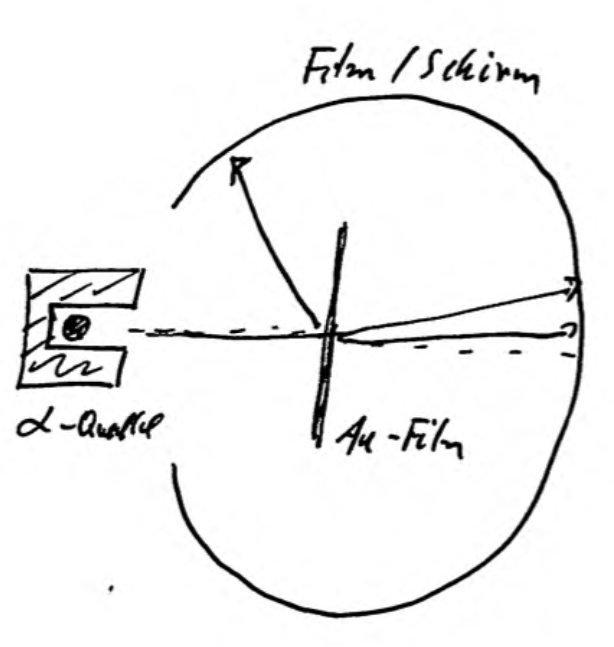
\includegraphics[width=\textwidth]{\currfiledir  sketch/rutherford.png}
    \caption{Skizze des Versuchsaufbaus von Rutherford}
\end{marginfigure}

Ernest Rutherford wollte 1911 dieses Modell überprüfen, indem er mit seinen Mitarbeitern Marsden und Geiger die kurz zuvor beim radioaktiven Zerfall entdeckten Alphateilchen auf eine dünne Goldfolie schoss. Alphateilchen bestehen aus zwei Protonen und zwei Neutronen, sind also doppelt positiv geladene Heliumkerne. Ihr Verhältnis $q/m$ war schon damals bekannt.

Nach dem Thomson-Modell würde man erwarten, dass die Alphateilchen nur wenig abgelenkt werden. Die Ladungen im Atom kompensieren sich und keine kann einen großen Effekt haben. Das sieht man auch, wenn man den transmittierten Alphastrahl auf einem Schirm beobachtet.



Die Überraschung war jedoch, dass einige Alphateilchen auch in sehr hohen Winkeln abgelenkt wurden, manche fast reflektiert. Das lässt sich mit dem Thomson-Modell nicht erklären. Dazu muss die Masse (und genügend positive Ladung) in einem viel kleineren Volumen als dem des Atoms konzentriert sein. Rutherford hatte den Atomkern entdeckt. Die positive Ladung und fast die gesamte Masse sind in dem sehr kleinen Atomkern mit einem Durchmesser von etwa \si{10^{-14}}{m} = \si{10}{fm} konzentriert. Der Rest des Atoms ist leer. Die Elektronen spielen für dieses Streuexperiment keine Rolle, da ihre Masse viel kleiner ist als die der Alphateilchen.

\begin{marginfigure}
    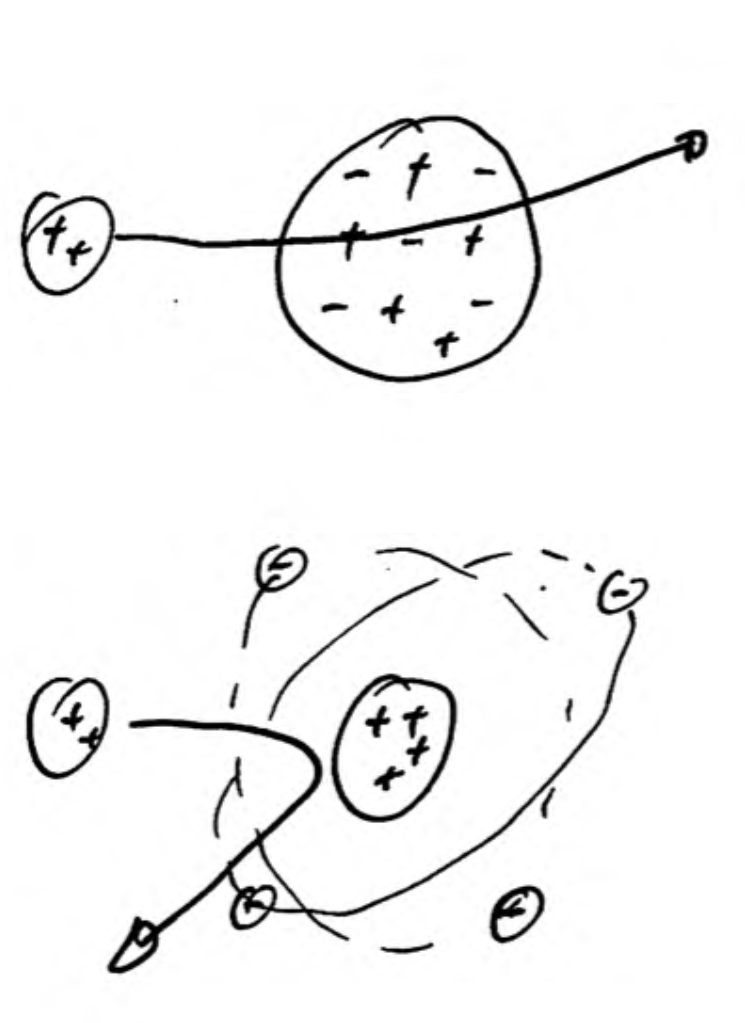
\includegraphics[width=\textwidth]{\currfiledir  sketch/atommodelle.png}
    \caption{Die Modelle von Thomson und  Rutherford sagen unterschiedliche Bahnen des  Alphateilchens vorbaus.}
\end{marginfigure}

\section{Rutherfordsche Streuformel}

Im Rutherford-Experiment wird die Anzahl $N(\theta)$ der um den Winkel $\theta$ abgelenkten Alphateilchen gemessen. Dabei ist die Größe des Detektors zu berücksichtigen, die durch den Raumwinkel $d\Omega$ beschrieben wird. Die Streueffizienz wird durch den integralen Streuquerschnitt $\sigma$ bzw. durch den differentiellen Streuquerschnitt  
\begin{equation}
    \frac{d \sigma(\theta)}{d\Omega} = \frac{N(\theta)}{N_0}
\end{equation}
beschrieben, mit der Gesamtzahl $N_0$ aller Alphateilchen.




Das Rutherford-Modell kann rein klassisch modelliert werden. Man beschreibt die Bahn eines geladenen Teilchens im Coulombpotential einer punktförmigen geladenen Masse unter Berücksichtigung der Energie- und Impulserhaltung. Da das Problem rotationssymmetrisch um die Achse Alpha-Quelle -- Atomkern ist, wird nur der sogenannte Stoßparameter $b$ berücksichtigt, der den Abstand der nicht abgelenkten Bahn des Alpha-Teilchens von dieser Symmetrieachse angibt. Man findet\sidenote{dies ist eine Übungsaufgabe}  eine charakteristische $\sin^{-4} (\theta/2)$-Abhängigkeit:
\begin{equation}
    \frac{d \sigma(\theta)}{d\Omega} =
    \frac{1}{4} \left(
\frac{qQ}{4 \pi \epsilon_0 \; 2 E_{kin}}
    \right)^2 \, \frac{1}{\sin^4 (\theta/2)}
\end{equation}
wobei $Q$ und $q$ die Ladungen des Kerns und des Alphateilchens und $E_{kin}$ die kinetische Energie des weit vom Kern entfernten Alphateilchens sind.

\begin{marginfigure}
    \includegraphics[width=\textwidth]{\currfiledir rutherford_data.png}
    \caption{Verteilung der Auftreffpunkte der Alpha-Teilchen auf einem Film im Rutherford-Versuch. Die horizontale Koordinate entspricht dem Ablenkwinkel.}
\end{marginfigure}


\begin{questions}  
    \item Experimentieren Sie mit der Simulation\phet{rutherford_scattering} und erklären Sie Ihre Beobachtungen.
    \item Wie ändert sich die Geschwindigkeit des Alpha-Teilchens zwischen Quelle und Detektor? Oder bleibt sie gleich?
\end{questions}

    

\section{Elektronenvolt}

Nun ist es an der Zeit, die sehr praktische Einheit 'Elektronenvolt' einzuführen. Die Angabe einer Energie in Joule ist für makroskopische Fragestellungen sinnvoll. Deshalb wurde diese Einheit eingeführt. Für Objekte wie Atome und Kerne ist sie nicht mehr geeignet. 

Wir verwenden hier die Einheit 'Elektronenvolt', abgekürzt 'eV'. Sie beschreibt die Energie $\Delta E$, die ein Elektron aufgenommen hat, wenn es eine Potentialdifferenz von $\Delta U =1$~V durchlaufen hat, also 
\begin{equation}
    \Delta E = e \Delta U \quad \text{und somit} \quad \si{1}{eV} = \si{1.60 10^{-19}}{J} \quad .
\end{equation} 

Hier ist in mehrfacher Hinsicht Vorsicht geboten: Die Einheit besteht aus zwei Zeichen (wie Pa), was insbesondere in Kombination mit Kilo-, Mega-, etc. zunächst ungewohnt sein kann: \si{1}{keV} = \si{1000}{eV}. Und das 'V' von Volt taucht auf, ohne dass eine Spannung beschrieben wird. Da \si{1}{J} = \si{1}{VAs} ist \si{1}{eV} = \si{1.60 10^{-19}}{VAs}, aber die beiden V haben eine unterschiedliche Bedeutung.


\section{Aufbau des Atomkerns}

Das Periodensystem der Elemente wurde 1869 von Dmitri Mendelejew vorgeschlagen. Die Position eines Elements ergibt sich aus seiner Ordnungszahl $Z$, die immer eine ganze Zahl ist. Sie gibt auch an, wie viele Elektronen ein Atom besitzt und, da es insgesamt ladungsneutral sein muss, wie viele positiv geladene Protonen es besitzt. 

Aus der Chemie ist jedoch bekannt, dass die Masse von Elementen mit ähnlicher Ordnungszahl sehr unterschiedlich sein kann: Wasserstoff : Helium : Lithium geht in der Ordnungszahl 1:2:3, in der Masse aber wie 1:4:7.

Thomsons Experimente zur Masse geladener Ionen zeigten, dass chemisch identische Elemente mit unterschiedlichen Massen auftreten. Neon z.B. überwiegend mit der 20-fachen Masse des Wasserstoffs, in geringen Anteilen aber auch mit der 22-fachen und noch seltener mit der 21-fachen Masse.

Erst die Entdeckung des Neutrons im Jahr 1932 brachte Klarheit. Neutronen sind ungeladene Teilchen mit einer sehr ähnlichen Masse wie die Protonen. Die chemischen Elemente existieren in verschiedenen \emph{Isotopen}, die den gleichen Platz im Periodensystem einnehmen (gleiche Ordnungszahl $Z$, d.h. gleiche Elektronen- bzw. Protonenzahl), aber unterschiedliche Massen, d.h. unterschiedliche Neutronenzahlen haben.

Man unterscheidet die Isotope nach ihrer Massenzahl $A = Z + N$ mit der Neutronenzahl $N$. Die oben genannten Neonisotope sind also \ch{^{20}Ne}, \ch{^{22}Ne} und \ch{^{21}Ne}. Die Ordnungszahl verbirgt sich im chemischen Symbol \ch{Ne}, da alle Neonatome immer 10 Protonen besitzen. Dieses $Z=10$ definiert den Namen 'Neon'.


\begin{questions}  
    \item Vollziehen Sie die hier angegeben Zahlenwerte im Periodensystem und in einer Isotopentafel nach! 
    \item Welche anderen Isotope von Neon gibt es?
\end{questions}

  

\section{Grenzen der klassischen Physik}

Die Ende des 19. und Anfang des 20. Jahrhunderts durchgeführten Experimente waren beeindruckend und zeigten den Aufbau der Atome. Vieles konnte jedoch nicht erklärt werden. Das Problem der diskreten Atomspektren und des breiten Schwarzkörperspektrums wurde bereits erwähnt. Aber auch das Rutherfordsche Atommodell hat einen Pferdefuß: Nach der Maxwellschen Theorie der Elektrodynamik müsste eine Ladung, die sich beschleunigt bewegt, eine Quelle elektromagnetischer Strahlung sein. Eine Kreisbewegung ist eine beschleunigte Bewegung, ein kreisendes Elektron müsste also Energie verlieren und in kürzester Zeit in den Atomkern stürzen. Dies scheint nicht der Fall zu sein, aber warum nicht?

\section{Zusammenfassung}

\textit{Schreiben Sie hier ihre persönliche Zusammenfassung des Kapitels auf. Konzentrieren Sie sich auf die wichtigsten Aspekte.}

\vspace*{10cm}


%--------------------


\printbibliography[segment=\therefsegment,heading=subbibliography]
